\begin{wrapfigure}[16]{r}{0.45\linewidth}
  \vspace{-2em}
  \begin{tikzfigure}[Schematic representation of the NASS added below the sample and the control architecture used]
  \label{fig:system_control}
  \centering
  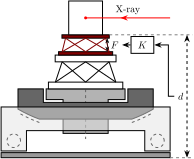
\includegraphics[width=0.9\linewidth]{./figs/system_control.pdf}


  \end{tikzfigure}
\end{wrapfigure}

\textbf{6 DoF Metrology System}
In order to achieve the positioning accuracy and stability requirements (shown on Table \ref{table:specifications}), a direct measurement of the relative position from the sample to the optical element is mandatory.
\emph{Laser interferometry} is chosen as it offers many advantages such as high resolution, high stability and large measurement range.

\vspace{1em}

\textbf{6 DoF Active Stabilization Stage}
In order to actively compensate the positioning error of the sample in all 6
DoF, a short stroke Stewart platform is added just below the sample as shown Figure~\ref{fig:system_control}.

By inverting the dynamics of the Stewart platform, it is possible to control independently the position of the mobile platform in all 6 DoF with respect to the fixed platform \cite{McInroy2000}.

\vspace{1em}

\textbf{Control Objective}
The control objective is to stabilize the position of the sample using the NASS actuators based on the 6DoF measurements provided by the metrology system.

Using this architecture, all the imperfections that cannot be compensated using the actual system (thermal drifts, guidance flexibilities, etc.) will be measured and compensated using a feedback control loop.

\vspace{1em}

\begin{minipage}[t]{0.63\linewidth}
  \textbf{Requirements For The NASS}
  The required stroke for the NASS should correspond to the maximum global
  positioning error of the end station without the NASS (\(\approx \SI{10}{\micro\metre}\) in translations).
  The repetability of the NASS is determined by the global specifications (Table \ref{table:specifications}).

  Other requirements such as stiffness and dynamical properties will be determined using the model presented below.
\end{minipage}
\begin{minipage}[t]{0.37\linewidth}
  \vspace{-1em}
  \begin{tikztable}[Rough estimation of the NASS specifications]
    \label{table:nass_specification}
    \centering
    \begin{tabular}{ccc}
      \toprule
      \textbf{Motion} & \textbf{Stroke} & \textbf{Repetability}\\
      \midrule
      \(T_{xyz}\) & \(\SI{\pm 10}{\micro\metre}\) & \(\SI{10}{\nano\metre}\)\\
      \(\theta_{xyz}\) & \(\SI{\pm 10}{\micro\radian}\) & \(\SI{1.7}{\micro\radian}\)\\
      \bottomrule
    \end{tabular}
  \end{tikztable}
\end{minipage}


% \textbf{Model Based Design}
% Such positioning system with multiple stages is highly coupled and presents many physical effects such as wobble that are difficult to model with a simple model based on measurements.
% Therefore, we have chosen to develop a 3D finite mass model. The software used is Simscape which is a toolbox for modeling multidomain physical systems within the Simulink environment.

% Each stage is represented as a 3D rigid body connected with the other stages by joints. Springs and dampers are added to take into account the finite stiffness of the mechanical guidance.
% Actuators and sensors dynamics are also included in the model.
% Finally, sources of perturbation and noise such as ground motion and sensor noise are also modeled.

% Thanks to the individual identification of each stage, stiffness and damping representing the flexibilities can be tuned properly.

% This model has numerous utility.
% First, it allows to conduct simulations of experiments such as tomography. That will help us to attest the performances of the system and compare various control architecture.
% Second, it permits to study the effect of the sample mass on the mechanical behavior of the system and verify the robustness properties of the controlled system.
% Finally, this model will be of great help for designing the NASS. Indeed, many parameters have to be properly chosen such as geometric configuration, leg stiffness, actuator type and rotational joints.

% In the following, the NASS is modeled as a Stewart platform with a cubic configuration, voice coil linear actuators and ideal rotational joints.

%%% Local Variables: ***
%%% mode:latex ***
%%% TeX-master: "2018 - Student Day.tex"  ***
%%% End: ***